\documentclass{beamer}
\let\vec\mathbf
\mode<presentation>
\usepackage{amsmath}
\usepackage{amssymb}
%\usepackage{advdate}
\usepackage{adjustbox}
%\usepackage{subcaption}
\usepackage{enumitem}
\usepackage{multicol}
\usepackage{mathtools}
\usepackage{listings}
\usepackage{url}
\usetheme{Boadilla}
\usecolortheme{lily}
\setbeamertemplate{footline}
{
  \leavevmode%
  \hbox{%
  \begin{beamercolorbox}[wd=\paperwidth,ht=2.25ex,dp=1ex,right]{author in head/foot}%
    \insertframenumber{} / \inserttotalframenumber\hspace*{2ex} 
  \end{beamercolorbox}}%
  \vskip0pt%
}
\setbeamertemplate{navigation symbols}{}
\providecommand{\nCr}[2]{\,^{#1}C_{#2}} % nCr
\providecommand{\nPr}[2]{\,^{#1}P_{#2}} % nPr
\providecommand{\mbf}{\mathbf}
\providecommand{\pr}[1]{\ensuremath{\Pr\left(#1\right)}}
\providecommand{\qfunc}[1]{\ensuremath{Q\left(#1\right)}}
\providecommand{\sbrak}[1]{\ensuremath{{}\left[#1\right]}}
\providecommand{\lsbrak}[1]{\ensuremath{{}\left[#1\right.}}
\providecommand{\rsbrak}[1]{\ensuremath{{}\left.#1\right]}}
\providecommand{\brak}[1]{\ensuremath{\left(#1\right)}}
\providecommand{\lbrak}[1]{\ensuremath{\left(#1\right.}}
\providecommand{\rbrak}[1]{\ensuremath{\left.#1\right)}}
\providecommand{\cbrak}[1]{\ensuremath{\left\{#1\right\}}}
\providecommand{\lcbrak}[1]{\ensuremath{\left\{#1\right.}}
\providecommand{\rcbrak}[1]{\ensuremath{\left.#1\right\}}}
\theoremstyle{remark}
\newtheorem{rem}{Remark}
\newcommand{\sgn}{\mathop{\mathrm{sgn}}}

\providecommand{\res}[1]{\Res\displaylimits_{#1}} 
\providecommand{\norm}[1]{\lVert#1\rVert}
\providecommand{\mtx}[1]{\mathbf{#1}}

\providecommand{\fourier}{\overset{\mathcal{F}}{ \rightleftharpoons}}
%\providecommand{\hilbert}{\overset{\mathcal{H}}{ \rightleftharpoons}}
\providecommand{\system}{\overset{\mathcal{H}}{ \longleftrightarrow}}
 %\newcommand{\solution}[2]{\textbf{Solution:}{#1}}
%\newcommand{\solution}{\noindent \textbf{Solution: }}
\providecommand{\dec}[2]{\ensuremath{\overset{#1}{\underset{#2}{\gtrless}}}}
\newcommand{\myvec}[1]{\ensuremath{\begin{pmatrix}#1\end{pmatrix}}}

\title{Matrices in Geometry - 7.4.42}
\author{EE25BTECH11035 Kushal B N}
\date{}

\begin{document}

\maketitle

\section{Problem Statement}
\begin{frame}
\frametitle{Problem Statement}
Find the intervals of values of $a$ for which the line $y+x = 0$ bisects two chords drawn from a point $\brak{\frac{1+\sqrt{2}a}{2},\frac{1-\sqrt{2}a}{2}}$ to the circle $2x^2 + 2y^2 - (1+\sqrt{2}a)x - (1-\sqrt{2}a)y = 0$.
\end{frame}

\section{Solution}
\begin{frame}{Solution}
Given,
Circle C: $x^2 + y^2 - \frac{1+\sqrt{2}a}{2}x - \frac{1-\sqrt{2}a}{2}y = 0$\\
Point $\vec{P} = \myvec{\frac{1+\sqrt{2}a}{2}\\\frac{1-\sqrt{2}a}{2}}$\\
Line L: $\vec{n}_L^{\top}\vec{x} = 0$, where $\vec{n}_L = \myvec{1\\1}$

The center of the circle is 
\begin{equation}
\vec{c} = \frac{1}{4}\myvec{1+\sqrt{2}a\\1-\sqrt{2}a}
\end{equation}
    
By observation,
\begin{equation}
    \vec{P} = 2\vec{c}
\end{equation}
The locus of midpoints, $\vec{M}$, of chords from $\vec{P}$ is given by,
\begin{equation}
    (\vec{M}-\vec{c})^{\top}(\vec{P}-\vec{M}) = 0
    \label{eq3}
\end{equation}
\end{frame}

\begin{frame}{Solution}
The midpoint $\vec{M}$ lies on the line L, the direction vector of which is
\begin{equation}
    \vec{m}_L = \myvec{1\\-1}
\end{equation}

\begin{equation}
\implies \vec{M} = \lambda\vec{m}_L
\end{equation}
Substituting this into equation \eqref{eq3}, we get
\begin{equation}
    (\lambda\vec{m}_L-\vec{c})^{\top}(\vec{P}-\lambda\vec{m}_L) = 0
\end{equation}
\begin{equation}
    \implies (\vec{m}_L^{\top}\vec{m}_L)\lambda^2 - \vec{m}_L^{\top}(\vec{P}+\vec{c})\lambda + \vec{c}^{\top}\vec{P} = 0
\end{equation}
\end{frame}

\begin{frame}{Solution}
For two distinct chords, the discriminant $\Delta = b^2 - 4ac > 0$.
\begin{equation}
    \Delta = \brak{\vec{m}_L^{\top}(\vec{P}+\vec{c})}^2 - 4\brak{\vec{m}_L^{\top}\vec{m}_L}\brak{\vec{c}^{\top}\vec{P}} > 0 \label{eq8}
\end{equation}
Here,
\begin{equation}
    \vec{m}_L^{\top}\vec{m}_L = \myvec{1&-1}\myvec{1\\-1} = 2
\end{equation}
\begin{equation}
    \vec{m}_L^{\top}(\vec{P}+\vec{c}) = \vec{m}_L^{\top}(3\vec{c}) = 3\myvec{1&-1}\frac{1}{4}\myvec{1+\sqrt{2}a\\1-\sqrt{2}a} = \frac{3\sqrt{2}a}{2}
\end{equation}
\begin{equation}
    \vec{c}^{\top}\vec{P} = 2\|\vec{c}\|^2 = \frac{1+2a^2}{4}
\end{equation}
\end{frame}

\begin{frame}{Solution}
Substituting into the inequality \eqref{eq8}:
\begin{equation}
    \brak{\frac{3\sqrt{2}a}{2}}^2 - 4(2)\brak{\frac{1+2a^2}{4}} > 0
\end{equation}
\begin{equation}
    \frac{9a^2}{2} - 2(1+2a^2) > 0
\end{equation}
\begin{equation}
    \frac{a^2}{2} > 2 \implies a^2 > 4
\end{equation}
\begin{equation}
    \implies a > 2 \quad \text{or} \quad a < -2
\end{equation}
\end{frame}

\section{Conclusion}
\begin{frame}{Conclusion}
The intervals of values for $a$ are $(-\infty, -2) \cup (2, \infty)$.
\begin{equation}
    \fbox{$a \in (-\infty, -2) \cup (2, \infty)$}
\end{equation}
\end{frame}

\begin{frame}{Plot}
\begin{figure}[H]
    \centering
    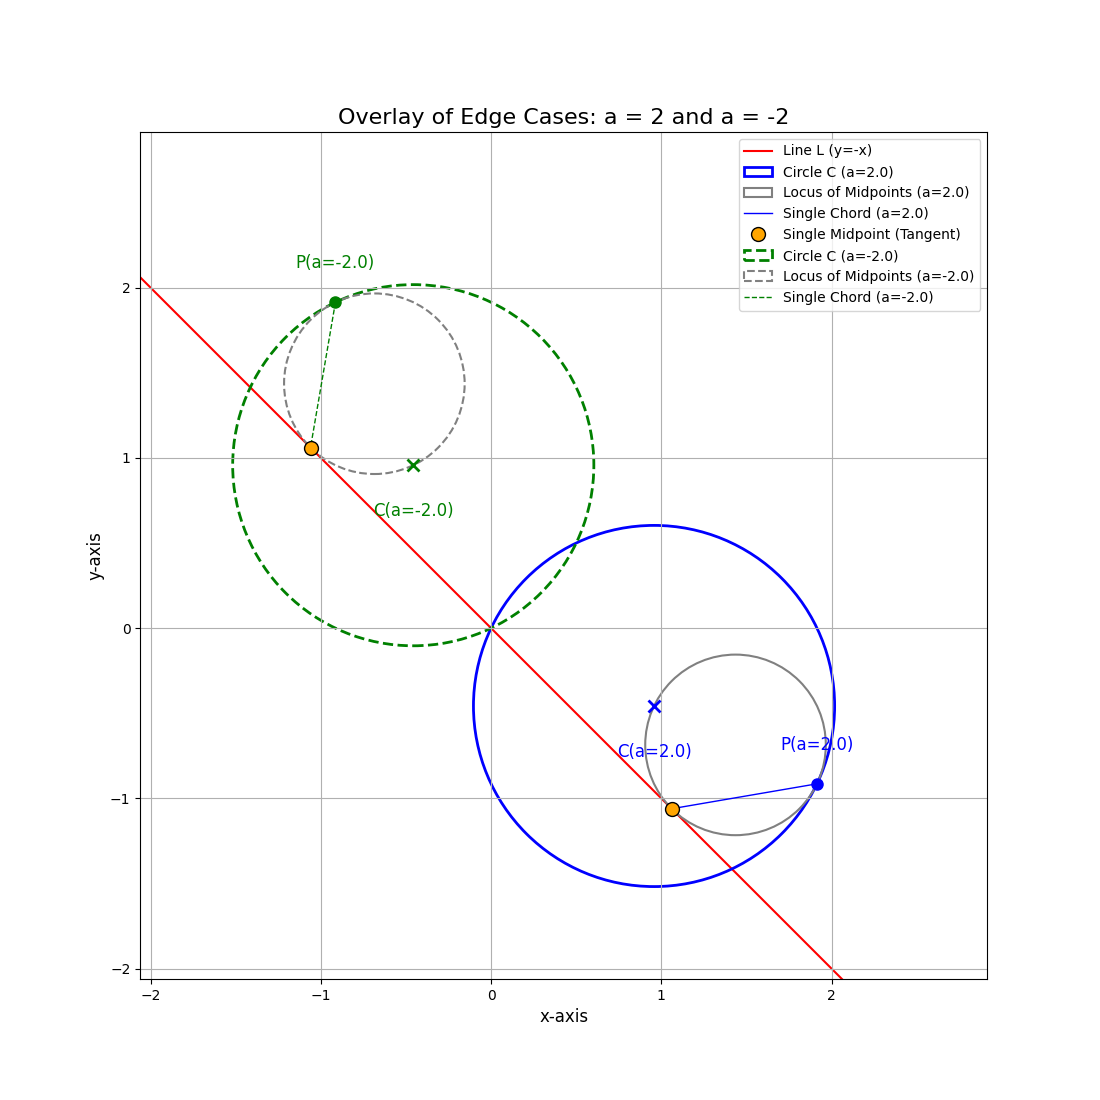
\includegraphics[width=0.60\columnwidth]{figs/fig.png}
    \caption{Plot for 7.4.42}
\end{figure}
\end{frame}

\end{document}
